\documentclass{standalone}

\usepackage{tikz-qtree}
\usepackage{circuitikz}
\usetikzlibrary{positioning,arrows}
\usepackage{rotating}
\newcommand{\random}[1]{\rotatebox[origin=c]{180}{$\mathsf{R}$}^{#1}} % randomized quantifier

\usetikzlibrary{automata}
\begin{document}
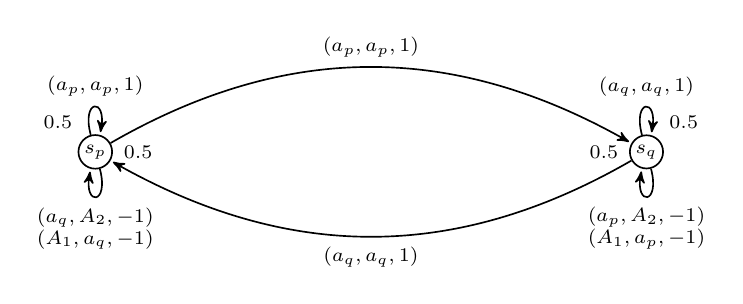
\begin{tikzpicture}[->,>=stealth',shorten >=1pt,auto,node distance=7cm,semithick]
    \tikzstyle{every node}=[font=\scriptsize]
    \node[state,inner sep=1pt,minimum size=0pt] (P) {$s_p$};
    \node[state,inner sep=1pt,minimum size=0pt] (Q) [right of=P] {$s_q$};
    \node[above left = 0.01 cm of P] {$0.5$};
    \node[right = 0.01 cm of P] {$0.5$};
    \node[above right = 0.01 cm of Q] {$0.5$};
    \node[left = 0.01 cm of Q] {$0.5$};

    \path
    (P) edge [bend left] node {$(a_p,a_p,1)$} (Q)
    edge [loop above] node {$(a_p,a_p,1)$} (P)
    edge [loop below] node[align=left] {$(a_q,A_2,-1)$\\$(A_1,a_q,-1)$} (P)
    (Q) edge [bend left] node {$(a_q,a_q,1)$} (P)
    edge [loop above] node {$(a_q,a_q,1)$} (Q)
    edge [loop below] node[align=left] {$(a_p,A_2,-1)$\\$(A_1,a_p,-1)$} (Q);
\end{tikzpicture}
\end{document}